% Этот шаблон документа разработан в 2014 году
% Данилом Фёдоровых (danil@fedorovykh.ru) 
% для использования в курсе 
% <<Документы и презентации в \LaTeX>>, записанном НИУ ВШЭ
% для Coursera.org: http://coursera.org/course/latex .
% Исходная версия шаблона --- 
% https://www.writelatex.com/coursera/latex/5.1

%\documentclass[t]{beamer}  % [t], [c], или [b] --- вертикальное выравнивание на слайдах (верх, центр, низ)
\documentclass[c, handout]{beamer} % Раздаточный материал (на слайдах всё сразу)
%\documentclass[aspectratio=169]{beamer} % Соотношение сторон

%\usetheme{Berkeley} % Тема оформления
%\usetheme{Bergen}
%\usetheme{Szeged}

%\usecolortheme{beaver} % Цветовая схема
%\useinnertheme{circles}
%\useinnertheme{rectangles}

\usetheme{Boadilla}
\usecolortheme{dolphin}

%%% Работа с русским языком
\usepackage{cmap}					% поиск в PDF
\usepackage{mathtext} 				% русские буквы в формулах
\usepackage[T2A]{fontenc}			% кодировка
\usepackage[utf8]{inputenc}			% кодировка исходного текста
\usepackage[english,russian]{babel}	% локализация и переносы

%%% Дополнительная работа с математикой
\usepackage{amsmath,amsfonts,amssymb,amsthm,mathtools} % AMS
\usepackage{icomma} % "Умная" запятая: $0,2$ --- число, $0, 2$ --- перечисление

%% Номера формул
%\mathtoolsset{showonlyrefs=true} % Показывать номера только у тех формул, на которые есть \eqref{} в тексте.
%\usepackage{leqno} % Нумерация формул слева

%% Свои команды
\DeclareMathOperator{\sgn}{\mathop{sgn}}
\DeclareMathOperator{\cov}{Cov}
\let\P\relax
\DeclareMathOperator{\P}{\mathbb{P}}
\DeclareMathOperator{\E}{\mathbb{E}}
\DeclareMathOperator{\Var}{Var}

%% Перенос знаков в формулах (по Львовскому)
\newcommand*{\hm}[1]{#1\nobreak\discretionary{}
	{\hbox{$\mathsurround=0pt #1$}}{}}

%%% Работа с картинками
\usepackage{graphicx}  % Для вставки рисунков
\graphicspath{{images/}{images2/}}  % папки с картинками
\setlength\fboxsep{3pt} % Отступ рамки \fbox{} от рисунка
\setlength\fboxrule{1pt} % Толщина линий рамки \fbox{}
\usepackage{wrapfig} % Обтекание рисунков текстом

%%% Работа с таблицами
\usepackage{array,tabularx,tabulary,booktabs} % Дополнительная работа с таблицами
\usepackage{longtable}  % Длинные таблицы
\usepackage{multirow} % Слияние строк в таблице

%%% Программирование
\usepackage{etoolbox} % логические операторы

%%% Другие пакеты
\usepackage{lastpage} % Узнать, сколько всего страниц в документе.
\usepackage{soul} % Модификаторы начертания
\usepackage{csquotes} % Еще инструменты для ссылок
%\usepackage[style=authoryear,maxcitenames=2,backend=biber,sorting=nty]{biblatex}
\usepackage{multicol} % Несколько колонок

%%% Картинки
\usepackage{tikz} % Работа с графикой
\usepackage{pgfplots}
\usepackage{pgfplotstable}

\DeclareMathOperator{\Lin}{\mathrm{Lin}}
\DeclareMathOperator{\Linp}{\Lin^{\perp}}
\DeclareMathOperator*\plim{plim}
%\DeclareMathOperator{\grad}{grad}
\DeclareMathOperator{\card}{card}
%\DeclareMathOperator{\sgn}{sign}
\DeclareMathOperator{\sign}{sign}

\DeclareMathOperator*{\argmin}{arg\,min}
\DeclareMathOperator*{\argmax}{arg\,max}
\DeclareMathOperator*{\amn}{arg\,min}
\DeclareMathOperator*{\amx}{arg\,max}
%\DeclareMathOperator{\cov}{Cov}
%\DeclareMathOperator{\Var}{Var}
\DeclareMathOperator{\Cov}{Cov}
\DeclareMathOperator{\Corr}{Corr}
\DeclareMathOperator{\pCorr}{pCorr}

\let\P\relax
\DeclareMathOperator{\P}{\mathbb{P}}



\newcommand{\cN}{\mathcal{N}}
\newcommand{\cU}{\mathcal{U}}
\newcommand{\cBinom}{\mathcal{Binom}}
\newcommand{\cPois}{\mathcal{Pois}}
\newcommand{\cBeta}{\mathcal{Beta}}
\newcommand{\cGamma}{\mathcal{Gamma}}

\def \R{\mathbb{R}}
\def \N{\mathbb{N}}
\def \Z{\mathbb{Z}}

\title[Введение в АД и статистику]{Введение в анализ данных и статистику}
%\subtitle{Monetary Policy in Terms of Capital Outflow}
\author[Омелюсик В.С.]{Омелюсик Владимир Степанович}
\date{\today}
\institute[НИУ ВШЭ]{Национальный Исследовательский Университет \\ <<Высшая школа экономики>> \\ -- \\ Факультатив «Введение в анализ данных и машинное обучение на Python»}

\newcommand{\art}[1]{({\small\textit{#1}})}

\usepackage{hyperref}
\hypersetup{urlcolor=blue,  colorlinks=true, linkcolor=black}

\usepackage{listings}    


\lstset{ 
	language=R,                     % the language of the code
	basicstyle= \ttfamily, % the size of the fonts that are used for the code
	%numbers=left,                   % where to put the line-numbers
	%numberstyle=\tiny\color{blue},  % the style that is used for the line-numbers
	%stepnumber=1,                   % the step between two line-numbers. If it is 1, each line
	% will be numbered
	%numbersep=5pt,                  % how far the line-numbers are from the code
	backgroundcolor=\color{white},  % choose the background color. You must add \usepackage{color}
	showspaces=false,               % show spaces adding particular underscores
	showstringspaces=false,         % underline spaces within strings
	showtabs=false,                 % show tabs within strings adding particular underscores
	%frame=single,                   % adds a frame around the code
	%rulecolor=\color{teal},        % if not set, the frame-color may be changed on line-breaks within not-black text (e.g. commens (green here))
	tabsize=1,                      % sets default tabsize to 2 spaces
	captionpos=b,                   % sets the caption-position to bottom
	breaklines=true,                % sets automatic line breaking
	breakatwhitespace=false,        % sets if automatic breaks should only happen at whitespace
	keywordstyle=\color{black},      % keyword style
	commentstyle=\color{purple},   % comment style
	stringstyle=\color{violet}      % string literal style
} 


\begin{document}
	
	\frame[plain]{\titlepage}	% Титульный слайд
	
	\begin{frame}{Направления математики}
		\begin{itemize}\setlength\itemsep{1em}
			\item Линейная алгебра
			\item Математический анализ
			\item Дифференциальные уравнения
			\item Теория вероятностей
			\item $\ldots$
		\end{itemize}
		\end{frame}
	
	\begin{frame}{Теория вероятностей и математическая статистика}
		\begin{itemize}\setlength\itemsep{1em}
			\item<1-> Теория вероятностей:
				\begin{itemize}\setlength\itemsep{0.5em}
					\item Знаем модель некоторого явления.
					\item Можем посчитать вероятность наступления какого-то события.
					\item И другие параметры модели.
				\end{itemize}
			\item<2-> Математическая статистика:
				\begin{itemize}\setlength\itemsep{0.5em}
					\item Модель явления нам неизвестна.
					\item Но есть наблюдения над этим явлением – данные.
					\item Идея: оценить параметры модели по данным. 
				\end{itemize}
		\end{itemize}
	\end{frame}

	\begin{frame}{Пример: подбрасывание монетки}
		\begin{itemize}\setlength\itemsep{1em}
			\item<1-> Пусть мы знаем вероятность выпадения орла при подбрасывании монетки равна $\frac{1}{2}$. Запишем это так:
			\[
				\P\{\text{Выпадет орёл}\} = \dfrac{1}{2}.
			\]
			Сумма вероятностей должна равняться 1. Поэтому вероятность выпадения решки тоже равна $\frac{1}{2}$.
			\item<2-> Это наша модель, в которой мы знаем, чему равны вероятности выпадения орла и решки. В реальной жизни мы эти вероятности не знаем и никогда не узнаем.
		\end{itemize}
	\end{frame}

	\begin{frame}{Пример: подбрасывание монетки}
		\begin{itemize}
			\item<1-> Что делать, если мы хотим узнать эти вероятности? Попробуем получить их \textbf{оценки}. 
			\item<2-> Проведём эксперимент: попросим человека подбрасывать монетку 100 раз. Запишем результаты подбрасывания:
			\[
			\text{О, О, Р, О, Р, Р, Р, О \ldots О, Р}.
			\]
			\item<3-> Оценку вероятности выпадения орла можно рассчитать, например, таким образом: 
			\[
			\hat{\P}\{ \text{Выпадет орёл} \} = \dfrac{\text{Число раз, когда выпал орёл}}{\text{Общее число подбрасываний}}.
			\]
			\item<4-> Оценка вероятности равна доле. Можно показать, что при некоторых условиях $\hat{\P}$ является «хорошей» оценкой $\P$ (будем понимать «хорошей» пока на интуитивном смысле).
		\end{itemize}
	\end{frame}
	
	\begin{frame}{Пример: среднее число посетителей}
		\begin{itemize}
			\item<1-> Случайная величина – величина, значение которой зависит от результата случайного происшествия (не подчиняющегося какому-либо шаблону).
			\item<2-> Математическое ожидание – среднее значение случайной величины при проведении эксперимента много раз. Очень много раз. 
			\item<3-> Пусть случайная величина $X$ – число посетителей ресторана за один день. Пусть математическое ожидание $X$:
			\[
			\mathbb{E}(X) = 78.
			\]
		\end{itemize}
	\end{frame}

	\begin{frame}{Пример: среднее число посетителей}
		\begin{itemize}\setlength\itemsep{1em}
			\item<1-> Чтобы оценить математическое ожидание, будем записывать число посетителей в течение 100 дней:
			\[
			X_1, X_2, X_3 \ldots X_{100}.
			\]
			\item<2-> В качестве оценки математического ожидания рассчитаем среднее арифметическое по всем наблюдениям:
			\[
			\hat{\mathbb{E}}(X) = \dfrac{X_1 + X_2 + \ldots X_{100}}{100}.
			\]
			\item<3-> Оценка математического ожидания равна среднему. Можно показать, что при некоторых условиях $\hat{\mathbb{E}}$ является «хорошей» оценкой $\mathbb{E}$.
		\end{itemize}
	\end{frame}
		
	\begin{frame}{Зачем пытаться узнать параметры модели?}
	
	Для решения практических задач:
			\begin{itemize}\setlength\itemsep{1em}
					\item Банку, выдающему кредиты, необходимо знать, с какой вероятностью кредит могут не вернуть.
					\item Владельцу торговой сети необходимо знать, где открыть новый магазин. Среднее число людей, проходящих в конкретном месте за день, может быть полезной характеристикой. 
					\item Рекомендательная система должна определить, с какой вероятностью контент понравится пользователю, и предложить наиболее подходящий вариант. 
			\end{itemize}
	\end{frame}
	
	\begin{frame}{Данные}
		\begin{itemize}\setlength\itemsep{1em}
			\item Для получения оценок нам необходимы наблюдения (данные). \textbf{Качество оценки} сильно зависит от \textbf{качества данных}.  
			\item Откуда берутся данные? Вообще говоря, из генеральной совокупности.
		\end{itemize}
		\begin{block}{Генеральная совокупность}
			Совокупность всех мыслимых наблюдений, которые могли бы быть произведены при данном реализованном комплексе условий. 
		\end{block}
	\end{frame}

	\begin{frame}{Данные}
			\begin{block}{Выборка}
				Часть генеральной совокупности, используемая для проведения эксперимента.
			\end{block}
			Пример:
			\begin{itemize}\setlength\itemsep{1em}
				\item Оценить вероятность того, что случайно выбранный ученик Лицея НИУ ВШЭ изучает английский язык.
				\item<2-> Генеральная совокупность: все ученики Лицея НИУ ВШЭ.
				\item<3-> Выборка: 10-е классы Лицея НИУ ВШЭ.
			\end{itemize}
			
			
	\end{frame}

	\begin{frame}{Репрезентативность выборки}
		\begin{block}{Репрезентативность выборки}
			Способность выборки описывать свойства генеральной совокупности. 
		\end{block}
		\vspace{3pt}
		\begin{itemize}\setlength\itemsep{1em}
			\item Исследуем выборку, получаем среднее, оценки вероятностей и проч.
			\item Можем ли сказать, что генеральная совокупность имеет то же среднее, оценки вероятностей и проч.?
			\item Да, если выборка репрезентативна. 
		\end{itemize}
	\end{frame}

	\begin{frame}{Репрезентативность выборки}
		Чтобы быть репрезентативной, выборка должна быть:
		\begin{itemize}\setlength\itemsep{1em}
			\item \alert{Несмещённой} в том смысле, что в ней должны присутствовать те же классы, что и в генеральной совокупности, в тех же пропорциях. 
			
			\textbf{Продолжение примера:} если мы знаем, что в Лицее НИУ ВШЭ большинство изучает английский, но некоторые также изучают французский и немецкий, то в несмещённой выборке большинство лицеистов должны изучать английский, но также должны быть изучающие французский и немецкий.
			
			\item<2-> \alert{Достаточной по числу наблюдений} (чем больше, тем лучше). Это позволяет учесть больше информации и получить более точные оценки. 
		\end{itemize}
	\end{frame}

	\begin{frame}{Случайность выборки}
		Чтобы быть репрезентативной, выборка должна быть случайной:
			\begin{itemize}
				\item То есть данные должны быть собраны случайным образом.
				\item Участие экспериментатора должно быть минимальным.  
			\end{itemize}
			\vspace{7pt}
			
			Пример: исследуем зависимость числа людей, посмотревших фильм, от рейтинга фильма на «Кинопоиске».			
			\begin{itemize}
				\item Как сформировать случайную выборку? 
			\end{itemize}
	\end{frame}
	
	
	\begin{frame}{Как выглядит выборка?}
		\begin{itemize}
			\item А если мы хотим изучить зависимость от нескольких факторов? 
			\item Нужно включить в выборку несколько переменных!
		\end{itemize}
		Общий вид выборки – таблица «объекты-признаки» ($N$ – число наблюдений, $k$ – число признаков):
		\begin{center}
		\def\arraystretch{1.5}
		\begin{tabular}{l| c c c c c}
			\hline
			  & $X_1$ & $X_2$ & $X_3$ & \ldots & $X_k$ \\
			\hline
			$1$ && &&& \\
			$2$ &&&&&\\
			$3$ &&&&& \\
			$\vdots$ &&&&&\\
			$N$ &&&&&\\
		\end{tabular}
		\end{center}
	\end{frame}

	\begin{frame}{Про терминологию}
		\begin{itemize}
			\item<1-> \alert{Зависимая переменная} (target) – переменная, значение которой хотим предсказать (например, прибыль кафе):
			\[
			Y
			\]
			\item<2-> \alert{Признаки} или Объясняющие переменные (features) – переменные, при помощи которых хотим предсказать значение зависимой переменной (например, расстояние в метрах до станции метро, время года, координаты расположения кафе):
			\[
			X_1, X_2, \ldots X_k
			\]
			\item<3-> \alert{Наблюдения} или объекты (observations) – конкретная реализация зависимой и объясняемой переменной. Наблюдений $N$ штук. 
		\end{itemize}
	\end{frame}

	\begin{frame}{Пример: кафе}
		\begin{itemize}
			\item<1-> Исследуем зависимость прибыли кафе от расстояния в метрах до станции метро, времени года и координат расположения кафе. Формализуем:
			\begin{itemize}
				\item $Y$ – прибыль кафе за месяц в тысячах рублей.
				\item $X_1$ – расстояния в метрах до станции метро.
				\item $X_2$ – время года.
				\item $X_3$ – координаты расположения кафе.
			\end{itemize}
			\item<2-> Пусть нам удалось собрать всего три наблюдения. Тогда таблица «объекты-признаки» может выглядеть следующим образом (числа придуманы):
			\begin{center}
				\def\arraystretch{1.5}
				\begin{tabular}{l| c c c}
					\hline
					& $X_1$ & $X_2$ & $X_3$ \\
					\hline
					$1$ & 100 & Зима & (30, 76) \\
					$2$ & 40   & Зима & (21, 12) \\
					$3$ & 150 & Лето & (4, 49) \\
				\end{tabular}
			\end{center}
		\end{itemize}
	\end{frame}

	\begin{frame}{Типы признаков}
		\begin{itemize}\setlength\itemsep{1em}
			\item<1-> Вещественные признаки (абсолютные или относительные): $X_k \in \R$.
				\begin{itemize}
					\item Возраст, площадь класса.
				\end{itemize}
			\item<2-> Категориальные номинальные признаки: $X_k \in \{\text{неупорядоченное множество}\}$.
			\begin{itemize}
				\item Цвет, название города.
			\end{itemize}
			\item<3-> Категориальные ранговые признаки: $X_k \in \{\text{упорядоченное множество}\}$.
			\begin{itemize}
				\item Воинское звание, ступень образования.
			\end{itemize}
		\item<4-> Бинарные признаки: $X_k \in \{0, 1\}$.
		\begin{itemize}
			\item Материал, из которого сделан стол, – дерево? 
		\end{itemize}
		\end{itemize}
	\end{frame}

	\begin{frame}{Пример: типы признаков}
		Определить типы признаков следующей таблицы «объекты-признаки»:
		\begin{center}
			\def\arraystretch{1.5}
			\begin{tabular}{l| c c c c c c}
				\hline
				& $X_1$ & $X_2$ & $X_3$  & $X_4$ & $X_5$ & $X_6$ \\
				\hline
				$1$ & 110 & Россия & 13\% & Small & 0 & 13.5  \\
				$2$ & 90 & Россия & 10\% & Medium & 0 & 10  \\
				$3$ & 105 & Германия & 30\% & Medium & 1 & 20  \\
				$4$ & 92 & США & 11\% & Small & 1 & 18.9  \\
				$5$ & 114 & Россия & 11\% & Large & 0 & 10  \\
				$6$ & 90 & Франция & 5\% & Small & 1 & 19  \\
			\end{tabular}
		\end{center}
		$N =?$, $k = ?$.
	\end{frame}

	\begin{frame}{Визуализация выборки}
		\begin{itemize}\setlength\itemsep{1em}
			\item Мы можем с лёгкостью визуализировать количественные переменные, чтобы понять примерный вид зависимостей в данных. 
			\item Это важно для дальнейшей интерпретации адекватности моделей:
				\begin{itemize}
					\item Если на «хороших» данных точно видно, что зависимость положительная, а модель показывает отрицательную модель, то вероятно, что-то не так с моделью. 
				\end{itemize} 
		\end{itemize}
	\end{frame}

	\begin{frame}{Диаграмма рассеяния (scatter plot)}
		По осям отложены интересующие переменные (данные сгенерированы).
		\begin{center}
		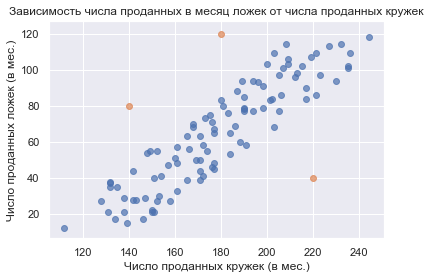
\includegraphics[width = 0.8\linewidth]{1.png}
		\end{center}
	\end{frame}

	\begin{frame}{Гистограмма (histogram)}
		По нижней оси отложены значения переменных, а по левой оси – частота встречаемости (данные сгенерированы).
		\begin{center}
			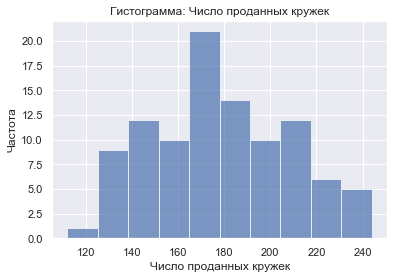
\includegraphics[width = 0.7\linewidth]{2.png}
		\end{center}
	\end{frame}

	\begin{frame}{Типы данных}
		\begin{itemize}
			\item<1-> \alert{Кроссекционные данные}: время фиксировано, зависимая переменная изменяется по объектам.
			
			\begin{center}
				\def\arraystretch{1.5}
				\begin{tabular}{l| c}
					\hline
					$N$ & $Y$ \\
					\hline
					$1$ & 10 \\
					$2$ & 40  \\
					$3$ & 100  \\
				\end{tabular}
			\end{center}
		
			\item<2-> Временные ряды: объект фиксирован, зависимая переменная изменяется во времени.
			
				\begin{center}
					\def\arraystretch{1.5}
					\begin{tabular}{l| c}
						\hline
						$t$ & $Y$ \\
						\hline
						$1$ & 100 \\
						$2$ & 40  \\
						$3$ & 150  \\
					\end{tabular}
				\end{center}
		\end{itemize}
	\end{frame}

	\begin{frame}{Типы данных}
			\begin{itemize}
				\item Панельные данные: зависимая переменная изменяется как по времени, так и по объектам. 
			\end{itemize}
			\begin{center}
				\def\arraystretch{1.5}
				\begin{tabular}{l| c| c}
					\hline
					$N$ & $t$ & $Y$ \\
					\hline
					$1$ & 1 & 100 \\
					$1$ & 2 & 120  \\
					$2$ & 1 & 150 \\
					$2$ & 2 & 152  \\
				\end{tabular}
			\end{center}
	\end{frame}

\end{document}